%   ------------------------------------------------------------------------
\FloatBarrier
\section{God Mode AI}
\label{s.godmodeAIApendice}

\begin{figure}[htbp]
    \centering
    \caption{\small Tela de converter a pixel art para alta resolução}
    \label{fig:godmodAIpixelto3D}
    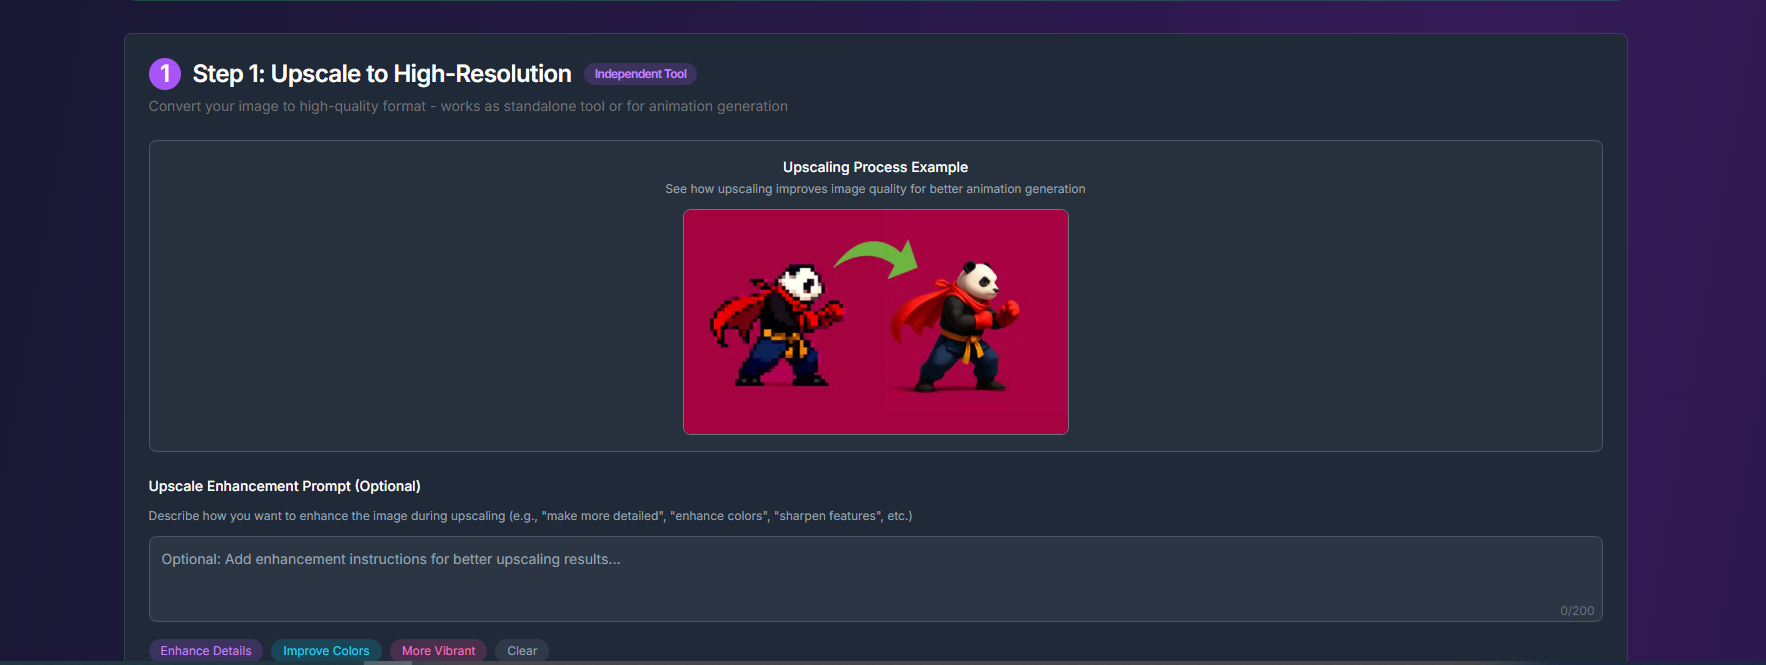
\includegraphics[width=1\linewidth]{figs/godmodAI/tela pixel art para 3D.PNG}
    \legend{\small Fonte: Elaborada pela autora.}
\end{figure}

\begin{figure}[htbp]
    \centering
    \caption{\small Tela para geração de animação}
    \label{fig:godmodAIGerarAnimacao}
    \begin{subfigure}{1\linewidth}
        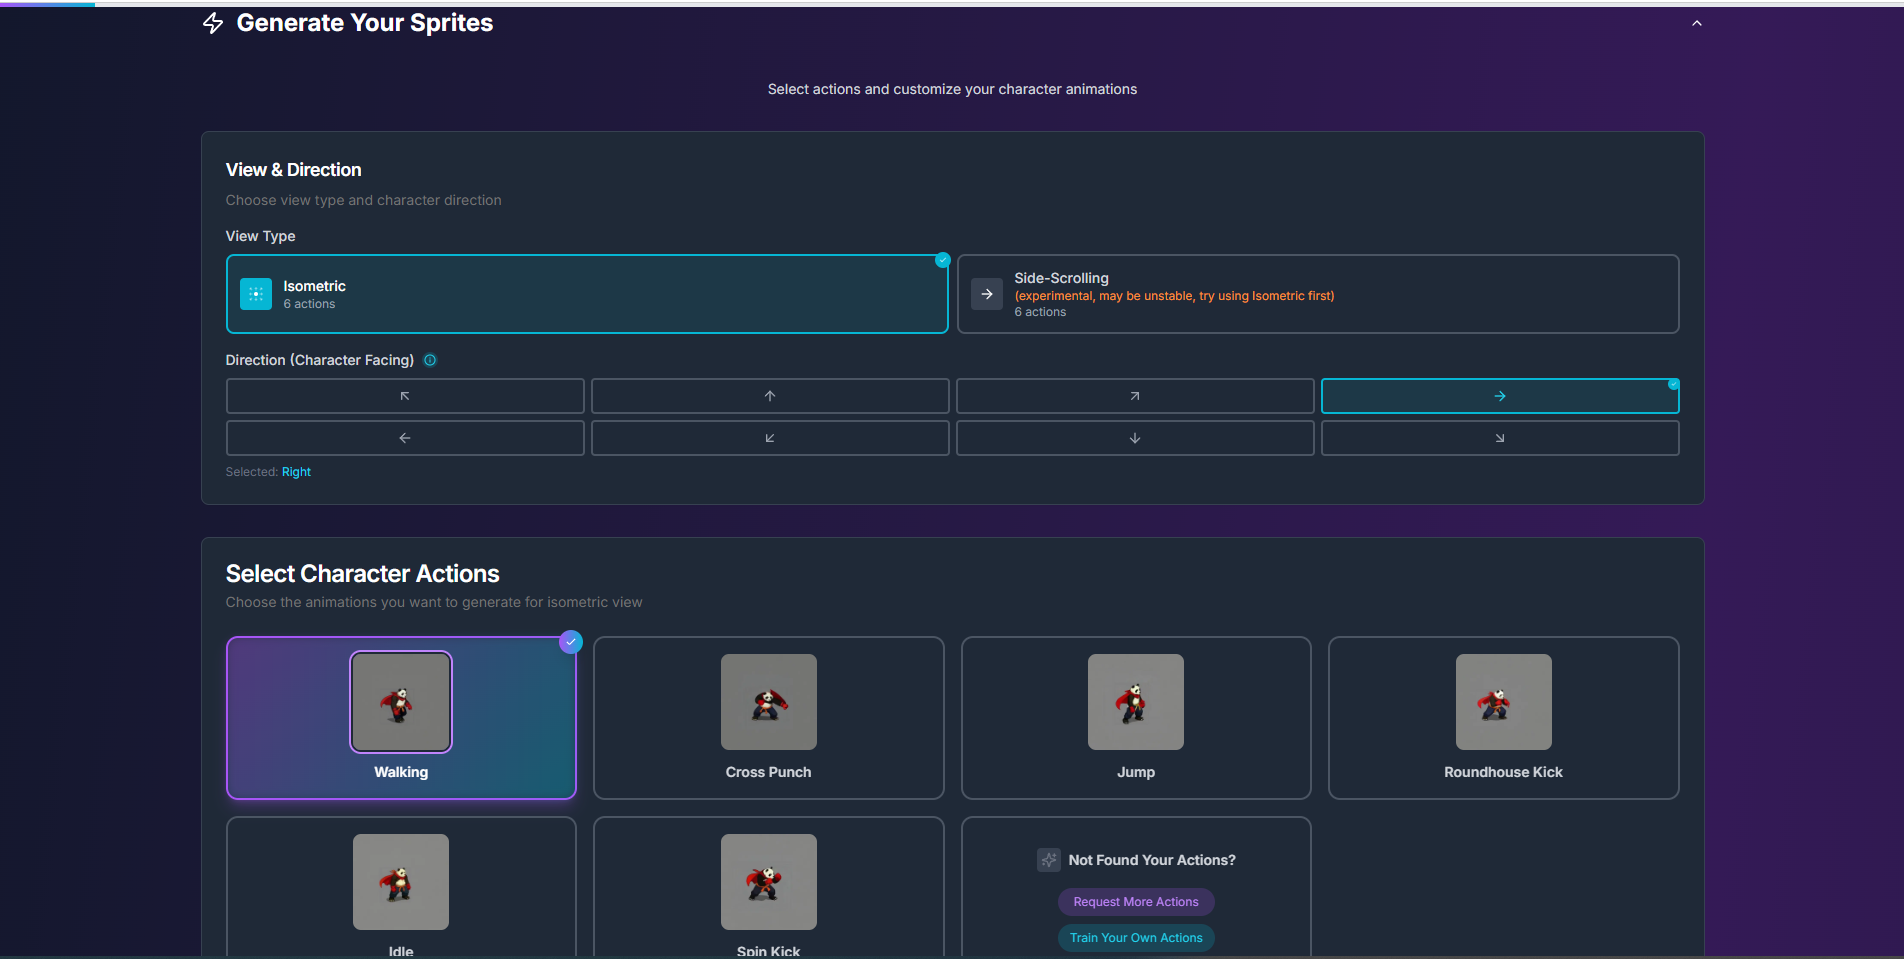
\includegraphics[width=1\linewidth]{figs/godmodAI/tela criando animação.PNG}
        \caption{\small Opções de ação e movimento.}
        \label{fig:godmodAIGerarAnimacao1}
    \end{subfigure}
    \legend{\small Fonte: Elaborada pela autora.}
    \begin{subfigure}{1\linewidth}
        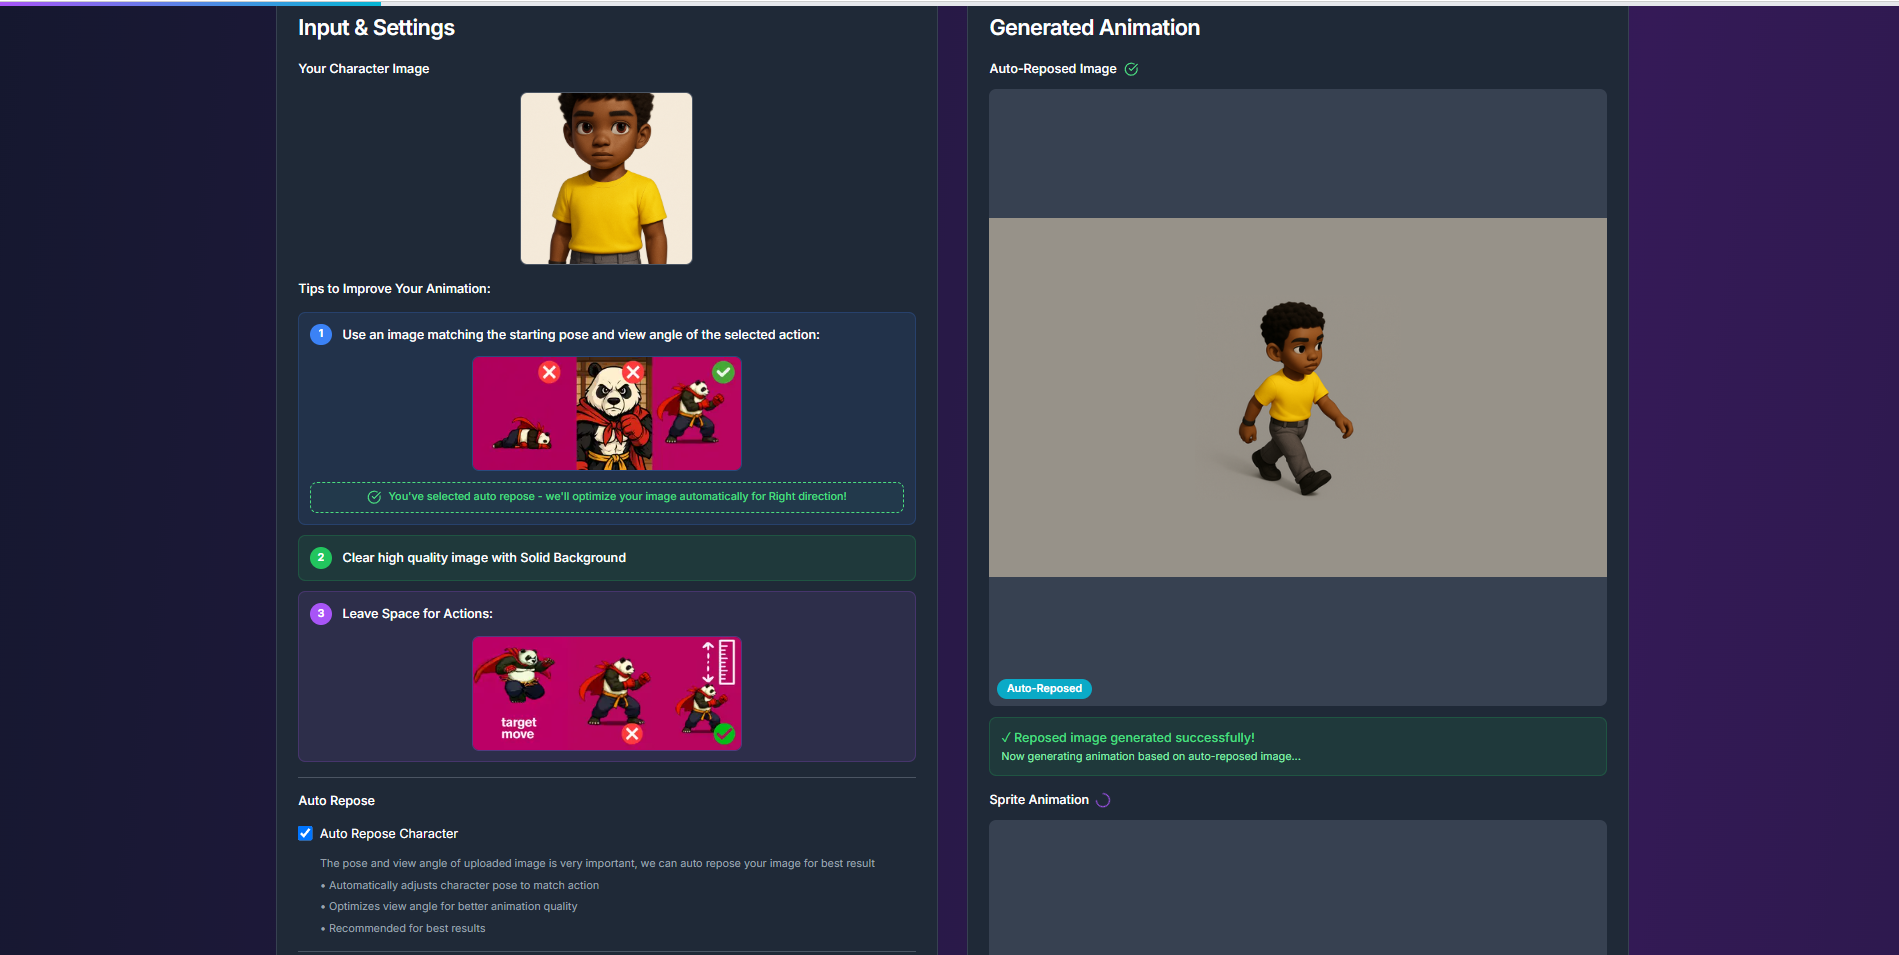
\includegraphics[width=1\linewidth]{figs/godmodAI/tela criando animação 2.PNG}
        \caption{\small Reposicionamento.}
        \label{fig:godmodAIGerarAnimacao2}
    \end{subfigure}
    \legend{\small Fonte: Elaborada pela autora.}
\end{figure}

\begin{figure}[htbp]
    \centering
    \caption{\small Tela de converter a animação para pixel art}
    \label{fig:godmodAI3Dtopixel}
    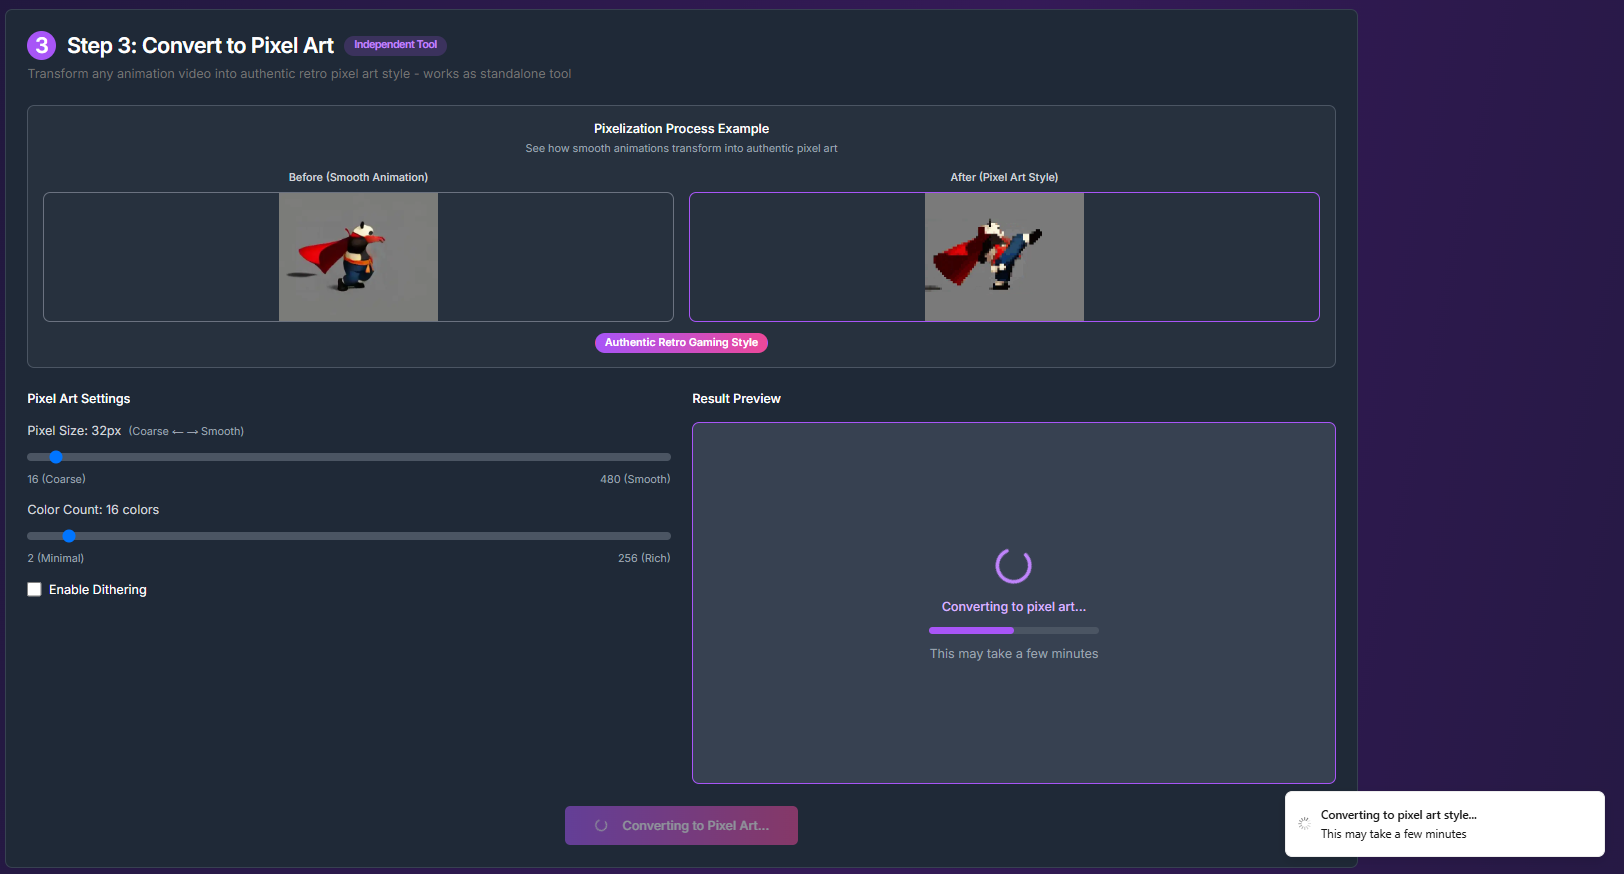
\includegraphics[width=1\linewidth]{figs/godmodAI/video para pixel art.PNG}
    \legend{\small Fonte: Elaborada pela autora.}
\end{figure}

\begin{figure}[htbp]
    \centering
    \caption{\small Interface nova}
    \label{fig:godmodModificado}
    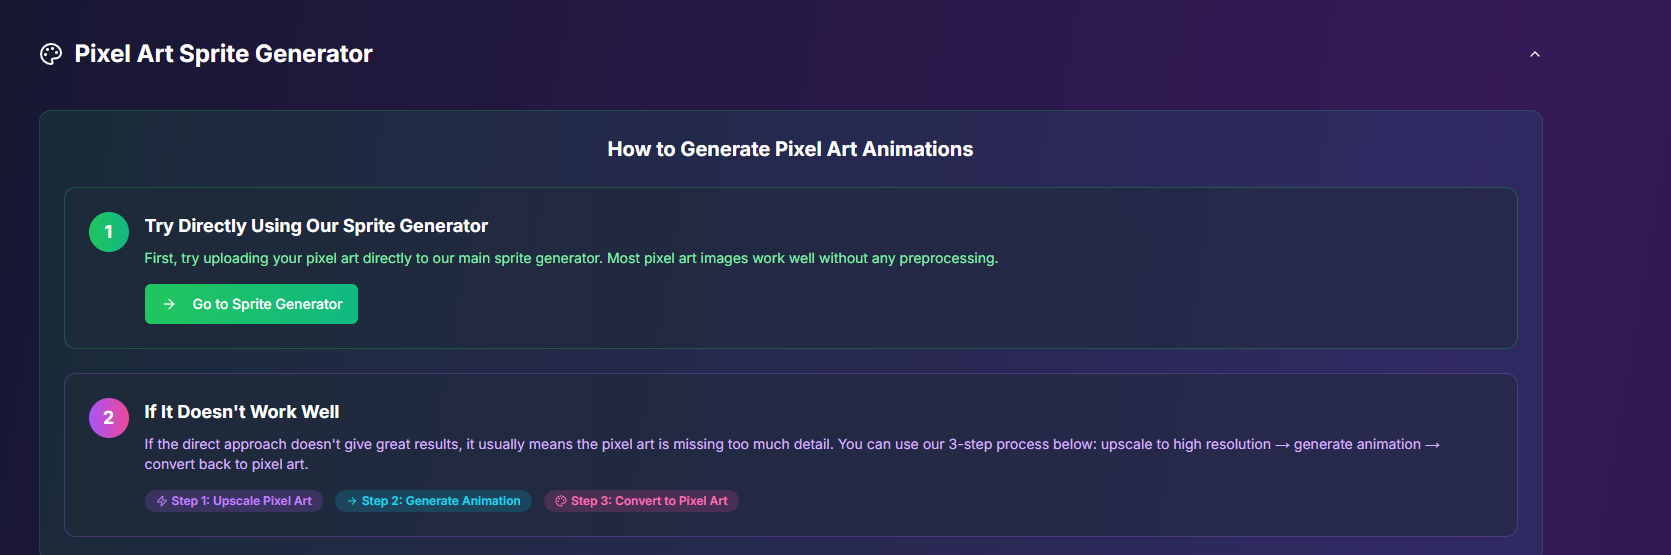
\includegraphics[width=1\linewidth]{figs/godmodAI/site modificado.PNG}
    \legend{\small Fonte: Elaborada pela autora.}
\end{figure}

\begin{figure}[htbp]
    \centering
    \caption{\small Auto reposicionamento no God Mode AI}
    \label{fig:godmodAIrepose}
    \begin{subfigure}{0.35\linewidth}
        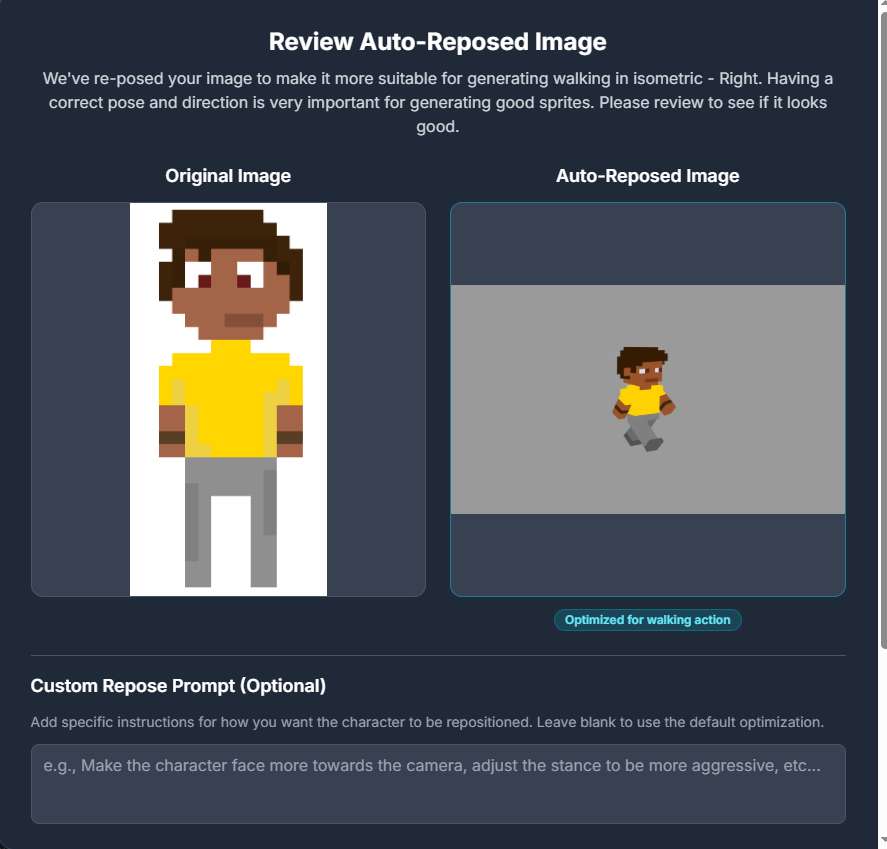
\includegraphics[width=1\linewidth]{figs/godmodAI/tela auto repose.PNG}
        \caption{\small Tentativa 1.}
        \label{fig:godmodAIrepose1}
    \end{subfigure}
    \begin{subfigure}{0.35\linewidth}
        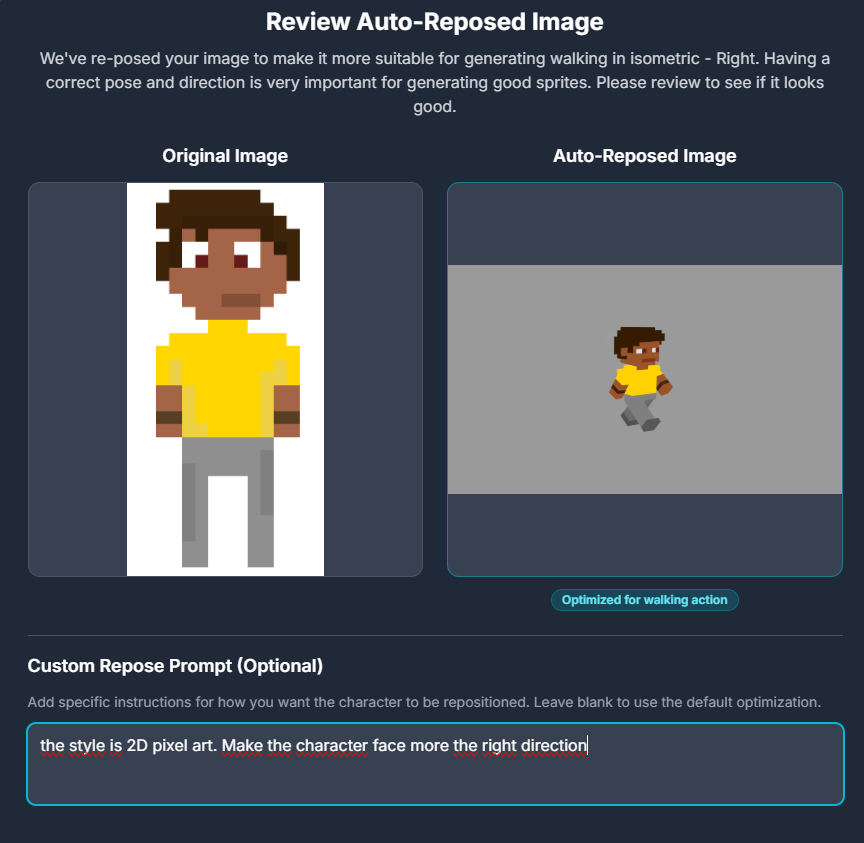
\includegraphics[width=1\linewidth]{figs/godmodAI/tela auto repose 2.PNG}
        \caption{\small Tentativa 2.}
        \label{fig:godmodAIrepose2}
    \end{subfigure}
    \begin{subfigure}{0.45\linewidth}
        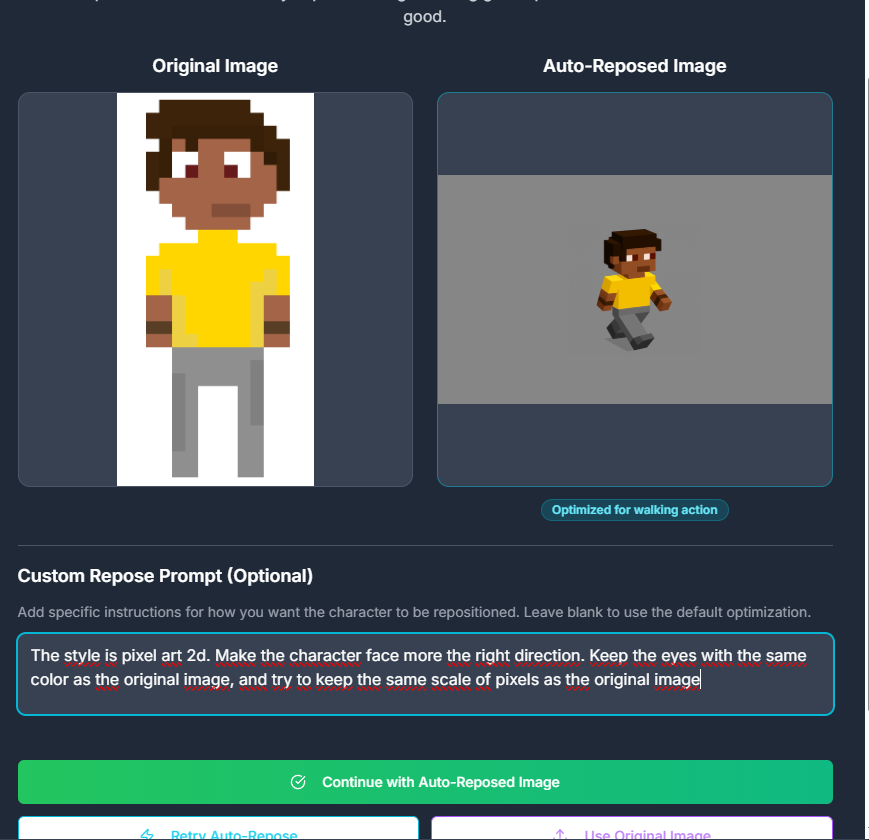
\includegraphics[width=1\linewidth]{figs/godmodAI/tela auto repose 3.PNG}
        \caption{\small Tentativa 3.}
        \label{fig:godmodAIrepose3}
    \end{subfigure}
        \begin{subfigure}{0.45\linewidth}
        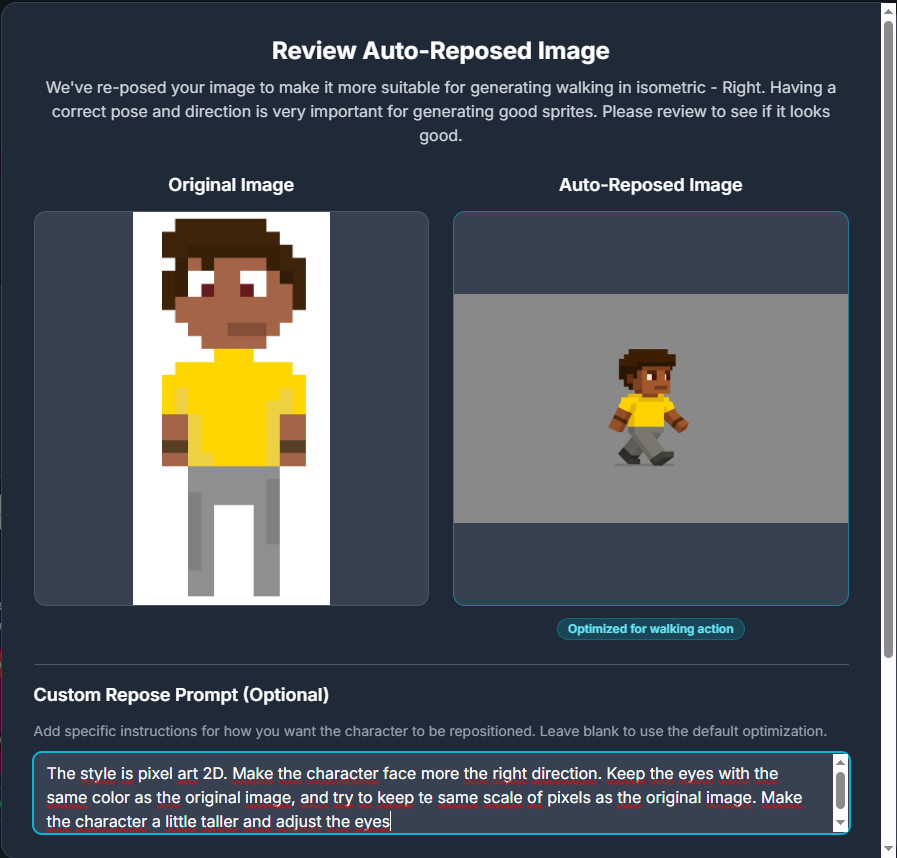
\includegraphics[width=1\linewidth]{figs/godmodAI/tela auto repose 4.PNG}
        \caption{\small Tentativa 4.}
        \label{fig:godmodAIrepose4}
    \end{subfigure}
        \begin{subfigure}{0.45\linewidth}
        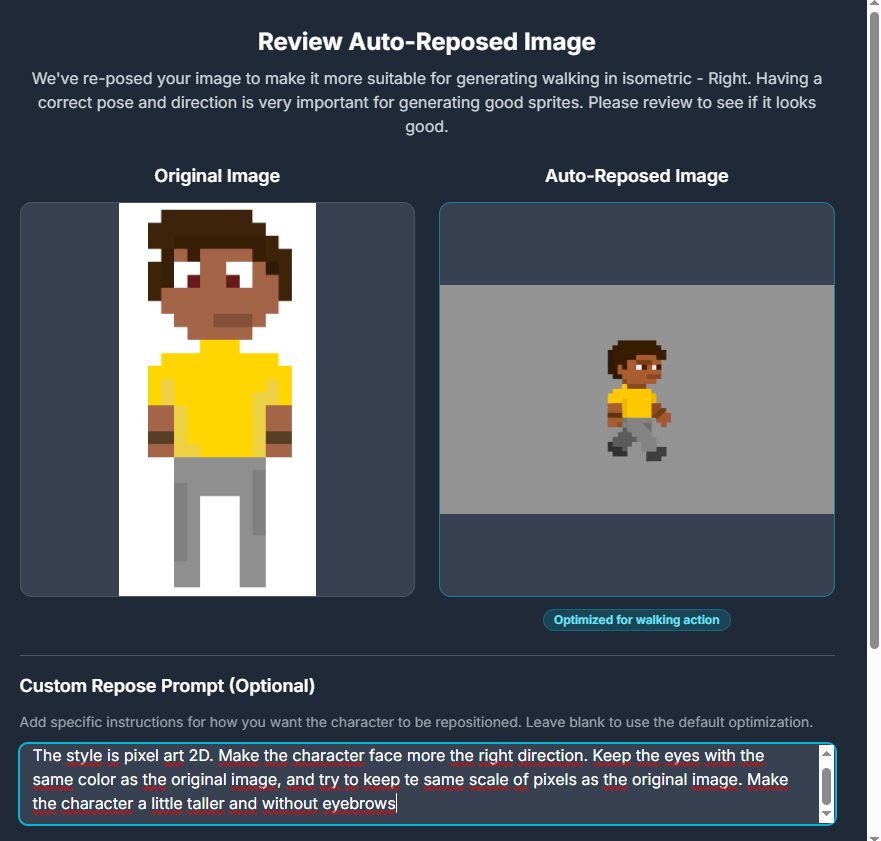
\includegraphics[width=1\linewidth]{figs/godmodAI/tela auto repose 5.PNG}
        \caption{\small Tentativa 5.}
        \label{fig:godmodAIrepose5}
    \end{subfigure}
        \begin{subfigure}{0.45\linewidth}
        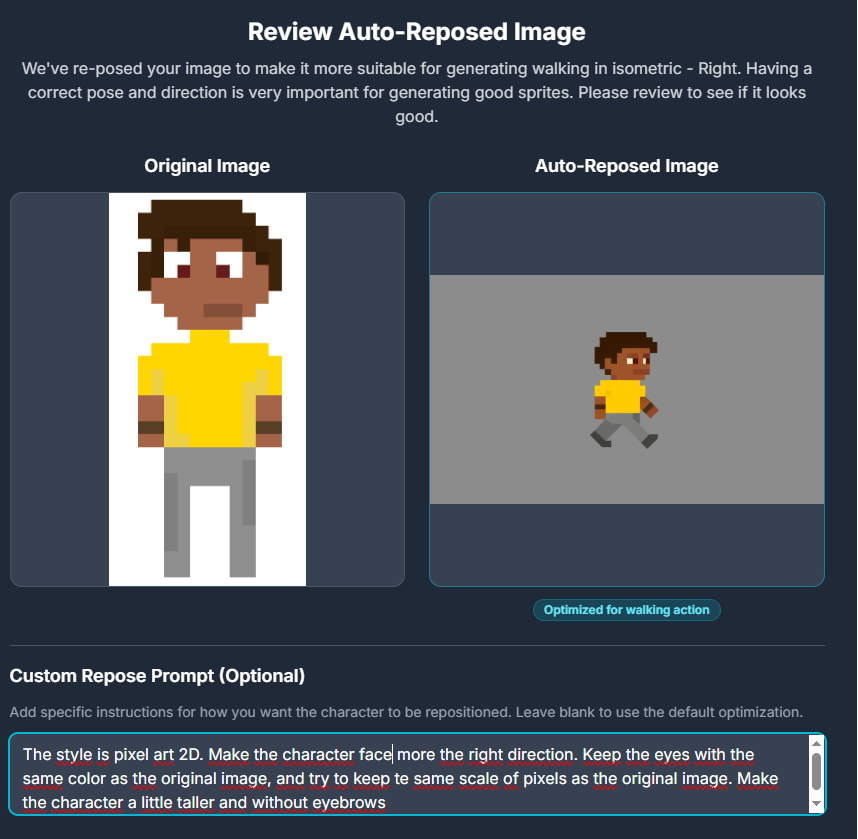
\includegraphics[width=1\linewidth]{figs/godmodAI/tela auto repose 6.PNG}
        \caption{\small Tentativa 6.}
        \label{fig:godmodAIrepose6}
    \end{subfigure}
    \legend{\small Fonte: Elaborada pela autora, utilizando a ferramenta God Mode AI.}
\end{figure}

\begin{figure}[htbp]
    \centering
    \caption{\small Tela de re-geração parcial}
    \label{fig:godmodAIregen}
    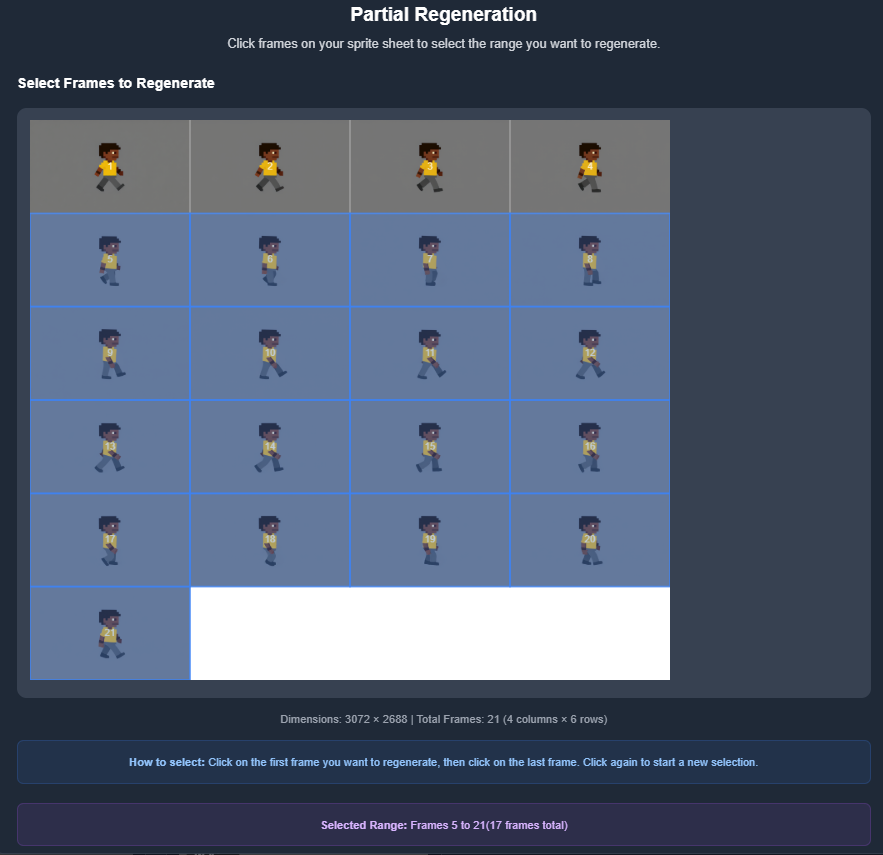
\includegraphics[width=1\linewidth]{figs/godmodAI/regeracao_parcial.PNG}
    \legend{\small Fonte: Elaborada pela autora.}
\end{figure}